%! Author = mariuszindel
%! Date = 02.11.20

\section{C\# Grundlagen}

\subsection{Überblick}
\subsubsection{Syntax}
Neue Code Features:
\begin{itemize}
    \item Referenzparameter
    \item Structs
    \item Blockmatratzen
    \item Enumerationstypen
    \item Uniformes Typsystem (int, long, etc.)
    \item goto $\rightarrow$ schlecht
    \item Systemnahes Programmieren
    \item Versionierung
\end{itemize}
Syntactic Sugar:
\begin{itemize}
    \item Komponentenunterstützung
    \begin{itemize}
        \item Properties
        \item Events
    \end{itemize}
    \item Delegates
    \item Indexers
    \item Boxing / Unboxing
\end{itemize}

\subsection{Sichtbarkeit}
\begin{tabular}{p{1cm} | p{7cm}}
    Attribut & Beschreibung\\
    \hline
    public & Überall sichtbar\\
    private & Innerhalb des jeweiligen Typen sichtbar\\
    protected & Innerhalb des jeweiligen Typen oder abgeleiteter Klasse sichtbar\\
    internal & Innerhalb des Assemblies sichtbar\\
    protected internal & Innerhalb des jeweiligen Typen, abgeleiteter Klasse oder Assemblies sichtbar\\
    private protected & Innerhalb des jeweiligen Typen, abgeleiteter Klasse wenn im gleichen Assemblie\\
\end{tabular}

\begin{tabular}{p{0.8cm} | p{0.8cm}| p{1cm}| p{0.8cm}| p{2.8cm}}
    Typ & Standart & Zulässig & Standart Members & Zulässig Members\\
    \hline
    class&internal&public/ internal&private& public protected internal private protectedinternal privateprotected\\
    struct&internal&public/ internal&private&public internal private\\
    enum&internal&public/ internal&public&-\\
    interface&internal&public/ internal&public&-\\
    delegate&internal&public/ internal&-&-\\
\end{tabular}

\subsection{Namespaces}

\begin{itemize}
    \item Entspricht in Java dem «Package»
    \item Beinhaltet
    \begin{itemize}
        \item Andere Namespaces
        \item Klassen
        \item Interfaces
        \item Structs
        \item Enums
        \item Delegates
    \end{itemize}
    \item Mehrere Namespaces in einem File möglich
    \item Namespace und Ordnerstruktur können sich unterscheiden
\end{itemize}
\begin{lstlisting}
//Es werden Namespaces importiert:
  using System;

//Namespaces werden in andere NS importiert:
namespace A
{ // gilt nur in dieser Datei fuer A
using C; }
namespace B { using D; }

//Alias-Namen moeglich
using F = System.Windows.Forms;
...
F.Button b;
\end{lstlisting}
\vspace{-10pt}
\begin{center}
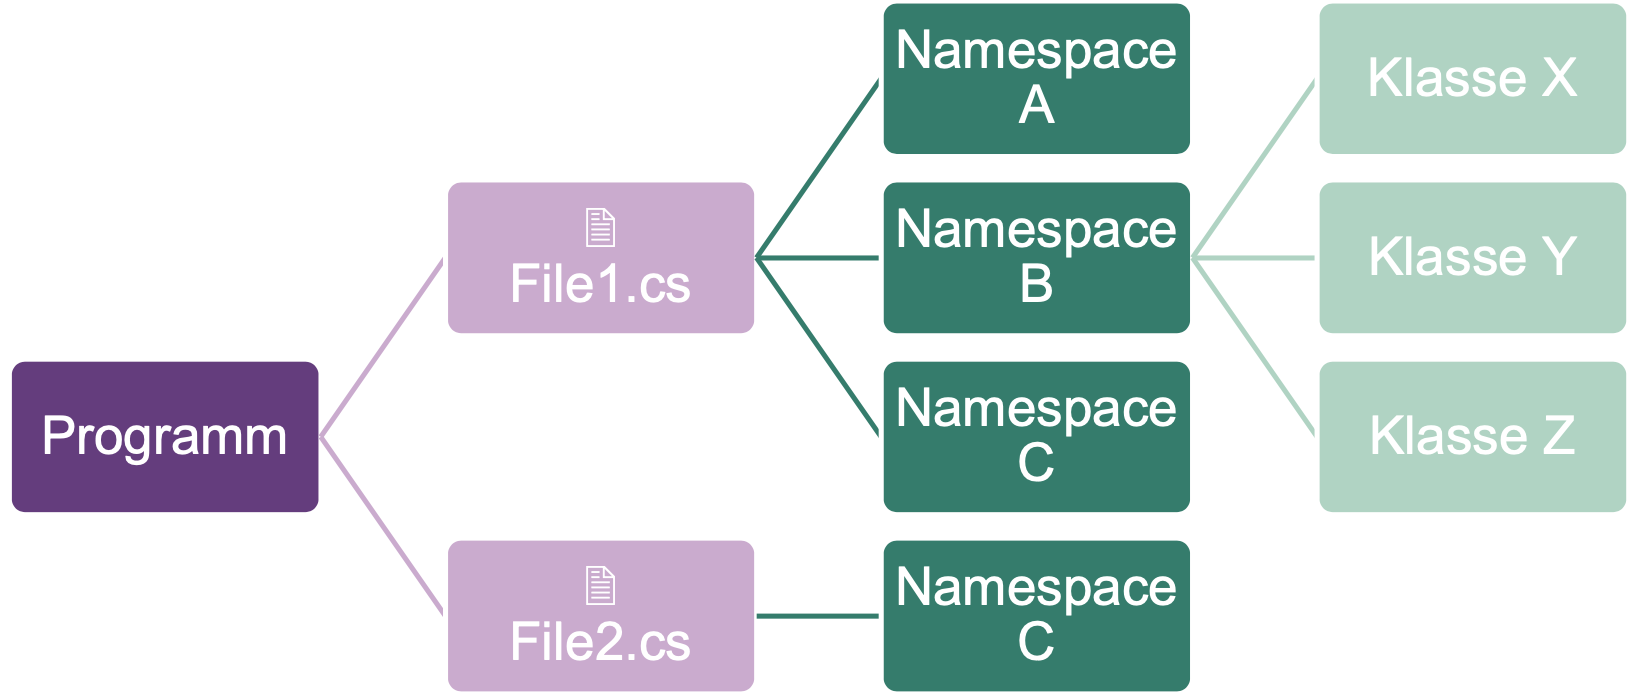
\includegraphics[scale=.21]{graphic/cGrundlagen/CGrundlagen_Aufteilung in Dateien.png}
\end{center}
\vspace{-8pt}

\subsection{Enumerationstypen}
Liste vordefinierter Konstanten inklusive Wert
\begin{lstlisting}
//Deklaration(leitet implizit von Int32 ab)
enum Days { Sunday, Monday, Tuesday, Wednesday, Thursday, Friday, Saturday };

// Verwendung:
Days today = Days.Monday;
if (today == Days.Monday) { /* ... */ } today = Days.Tuesday;
\end{lstlisting}

\subsubsection{Wertedefinition}
\begin{tabular}{l | l | l}
    Sunday&0&Erster Wert erhält 0\\
    Monday&1&Letzter Wert + 1\\
    Tuesday&2&Letzter Wert + 1\\
    Wednesday&3&Letzter Wert + 1\\
    Thursday&4&Letzter Wert + 1\\
    Friday&5&Letzter Wert + 1\\
    Saturday&6&Letzter Wert + 1\\
\end{tabular}
\begin{lstlisting}
// Werteauslesen/interpretieren(Int32)
int sundayValue = (int)Days.Sunday;

Console.WriteLine("{0} / #{1}.", Days.Sunday, sundayValue); // Ausgabe: Sunday / #0
int fridayValue = (int)Days.Friday;
Console.WriteLine("{0} / #{1}.", Days.Friday, fridayValue); // Ausgabe: Friday / #5
\end{lstlisting}

\subsubsection{explizite Wertedefinition}
\begin{lstlisting}
enum Days { Sunday = 10, Monday, Tuesday, Wednesday, Thursday, Friday = 9, Saturday };
\end{lstlisting}

\subsubsection{Basis-Typen}
Vergrössern / Verkleinern Wertebereich \& Speichernutzung:
\begin{lstlisting}
// Deklaration:
enum Days : byte { Sunday, Monday, Tuesday, Wednesday, Thursday, Friday, Saturday };
// Verwendung:
byte today = (byte)Days.Monday;
\end{lstlisting}

\subsubsection{Parsing}
Verwendung der Klasse «Enum»
\begin{lstlisting}
// String zu Enum parsen
Days day1 = (Days)Enum.Parse(typeof(Days), "Monday"); // Non-Generic (Exception on failure)
bool success3 = Enum.TryParse("Monday", out Days day3); // Generic / C# 7.0
\end{lstlisting}


\subsection{Arrays}
\subsubsection{Eindimensionale}
\begin{lstlisting}
int[] a = { 1, 3, 5 };

int length = array1.Length;

int value1 = array1[4];
\end{lstlisting}
\begin{center}
    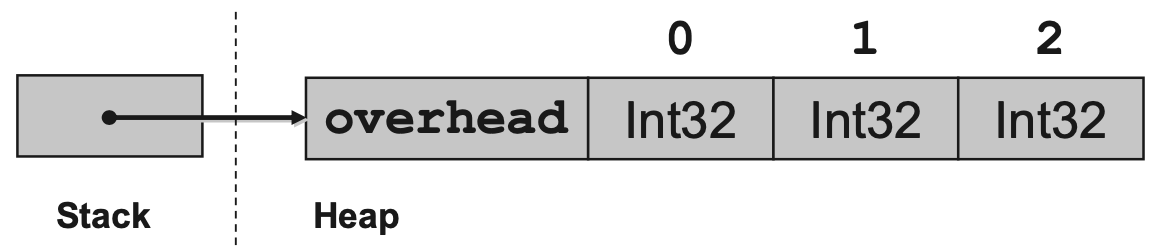
\includegraphics[scale=.23]{graphic/cGrundlagen/CGrundlagen_1Array_ValueTypes.png}
\end{center}
\vspace{-8pt}

\begin{lstlisting}
object[] a = new object[3]; a[1] = new object();
a[2] = 5;
\end{lstlisting}
\begin{center}
    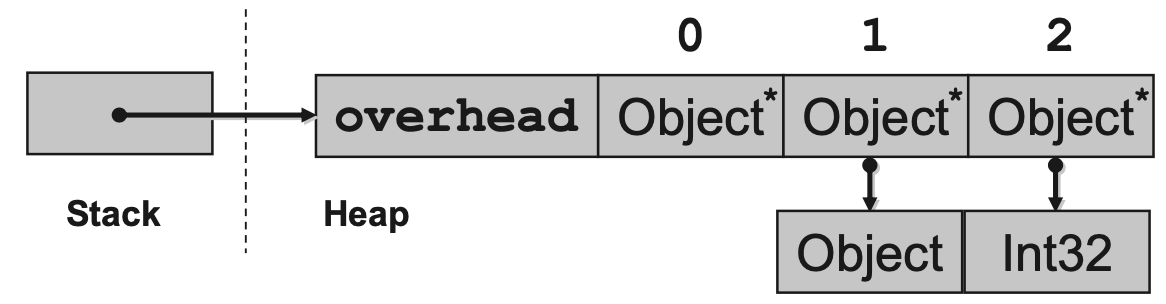
\includegraphics[scale=.23]{graphic/cGrundlagen/CGrundlagen_1Array_ReferenceTypes.png}
\end{center}
\vspace{-8pt}

\subsubsection{Mehrdimensionale (rechteckig / Blockmatritzen)}
\begin{lstlisting}
int[,] a = new int[3,2];
a[0,1] = 9; // Schreiben
int x = a[0,1]; // Lesen / Liefert 9

int length = a.Length; // Liefert 6
int length0 = a.GetLength(0); // Liefert 3
int length1 = a.GetLength(1);// Liefert 2
\end{lstlisting}
\begin{center}
    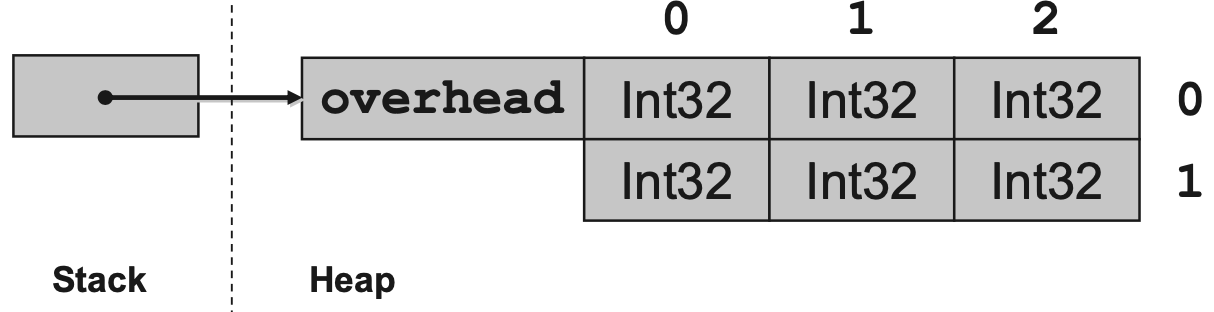
\includegraphics[scale=.23]{graphic/cGrundlagen/CGrundlagen_MArray_Rechteckig.png}
\end{center}
\vspace{-8pt}

\subsubsection{Mehrdimensionale (jagged)}
\begin{lstlisting}
int[][] a = new int[2][];
a[0] = new int[2];
a[1] = new int[1];
a[0][1] = 9; // Schreiben
int x = a[0][1]; // Lesen / Liefert 9

int length = a.Length; // Liefert 2
int length0 = a[0].Length; // Liefert 2
int length1 = a[1].Length; // Liefert 1
\end{lstlisting}
\begin{center}
    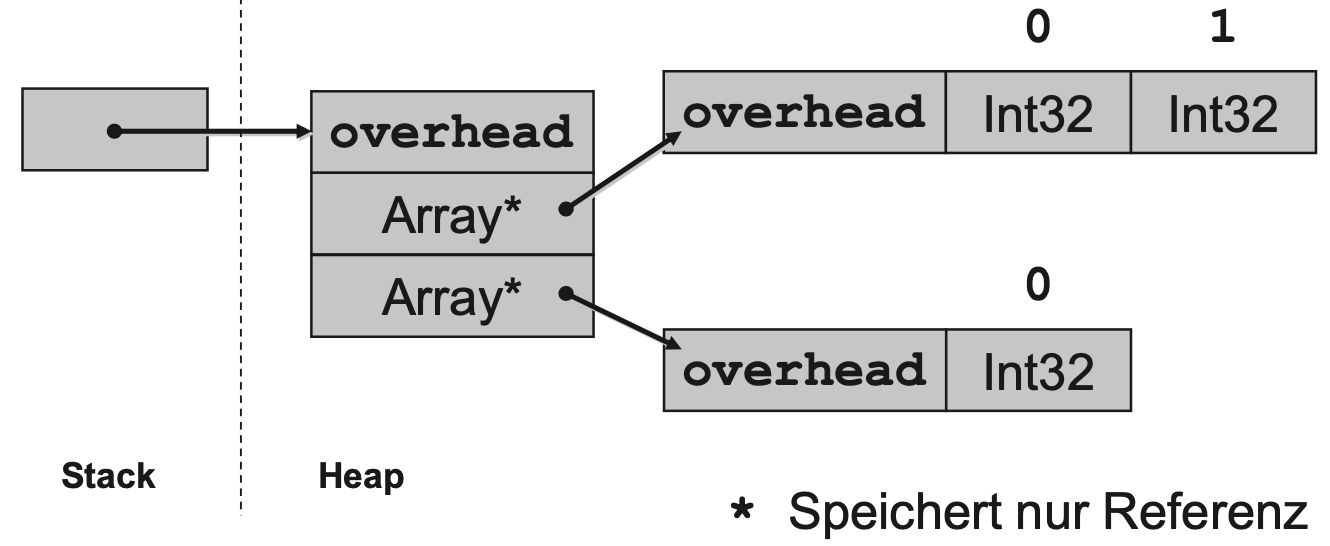
\includegraphics[scale=.23]{graphic/cGrundlagen/CGrundlagen_MArray_Jagged.png}
\end{center}
\vspace{-8pt}

\subsubsection{Vor-/Nachteile Blockmatritzen}
\begin{itemize}
    \item Speicherplatz-Effizienz
    \item SchnelleresAllozieren
    \item Schnellere Garbage Collection da «en bloc»
    \item Aber Boundary-Check wird bei 1-dimensionalen Arrays optimiert (gilt nicht für Blockmatrizen)
\end{itemize}

\subsection{Typkompatibilität}
\begin{center}
    \includegraphics[scale=.23]{graphic/cGrundlagen/CGrundlagen_Typkompatibilität.png}
\end{center}
\vspace{-8pt}

\subsection{Jumps}
\begin{itemize}
    \item break $\rightarrow$ Aktuellen Loop beenden
    \item continue $\rightarrow$ Zur nächsten Loop-Iteration
    \item goto «label» $\rightarrow$ Sprung zu «label»
\end{itemize}

\newpage